\onehalfspacing
\section{Đề số 22}
\graphicspath{{./img/}}
\begin{bt} 
    Thực hiện phép tính:
    \begin{enumerate}
        \item $A=1+5+5^2+5^3+5^4+\ldots+5^{2015}$
        \item $B=\frac{4^5 \cdot 9^4-2 \cdot 6^9}{2^{10} \cdot 3^8+6^8 \cdot 20}$
    \end{enumerate}
\loigiai{
    \begin{enumerate}
        \item Thực hiện phép tính\\[5px]
        $A=1+5^2+5^3+5^4+\ldots+5^{2015}$\\[5px] 
        Ta có:
$$
\begin{gathered}
5 \mathrm{~A}=5+5^2+5^3+5^4+\ldots+5^{2015}+5^{2016} \\[5px]
\mathrm{~A}=1+5+5^2+5^3+5^4+\ldots+5^{2015}
\end{gathered}
$$
Trừ theo vế : $5 \mathrm{~A}-\mathrm{A}=5^{2016}-1$
$$
\text {Vậy: } A=\frac{5^{2016}-1}{4}
$$
\item Ta có:\\[5px]
$\begin{aligned}
B & =\frac{4^5 \cdot 9^4-2 \cdot 6^9}{2^{10} \cdot 3^8+6^8 \cdot 20} \\[5px]
& =\frac{\left(2^2\right)^5 \cdot\left(3^2\right)^4-2 \cdot(2 \cdot 3)^9}{2^{10} \cdot 3^8+(2 \cdot 3)^8 \cdot 2^2 \cdot 5} \\[5px]
& =\frac{2^{10} \cdot 3^8-2^{10} \cdot 3^9}{2^{10} \cdot 3^8+2^{10} \cdot 3^8 \cdot 5} \\[5px]
& =\frac{2^{10} \cdot 3^8(1-3)}{2^{10} \cdot 3^8(1+5)} \\[5px]
& =-\frac{1}{3}
\end{aligned}$
    \end{enumerate}
}
\end{bt}

\begin{bt}
    \hfill
	\begin{enumerate}[a.]
        \item Tìm $x$ để biểu thức $\mathrm{P}=1+\frac{9}{3+|x-5|}$ đạt giá trị lớn nhất.
        \item Tìm giá trị của $x$ biết: $\quad|2 x-1|=2$.
        \item Cho 4 số $\mathrm{a}, \mathrm{b}, \mathrm{c}, \mathrm{d}$ trong đó $\mathrm{b}$ là trung bình cộng của a và $\mathrm{c}$ đồng thời $\frac{1}{c}=\frac{1}{2}\left(\frac{1}{b}+\frac{1}{d}\right)$.
        
        Chứng minh bốn số đó lập thành tỉ lệ thức.
    \end{enumerate}
	\loigiai{
        \begin{enumerate}
            \item Tìm $x$ để biểu thức $P=1+\frac{9}{3+|x-5|}$ đạt giá trị lớn nhất.\\[5px]
            Để $\mathrm{P}$ đạt giá trị lớn nhất khi $\frac{9}{3+|x-5|}$ đạt GTLN khi và chỉ khi
            $3+|x-5|$ đạt GTNN mà $|x-5| \geq 0$ dấu "=" khi $x=5$\\[5px]
            Vậy GTLN của $P=4$ khi $x=5$
            \item Tìm giá trị của $x$ biết : $|2 x-1|=2$.\\[5px]
            TH1: Xét với $2 x-1 \geq 0 \Rightarrow x \geq 0,5$ ta có:\\[5px]
            $|2 x-1|=2 \Rightarrow 2 x-1=2 \Rightarrow x=1,5$ (thỏa mãn đk)\\[5px]
            TH2: Xét với $2 x-1<0=>x<0,5$ ta có\\[5px]
            $|2 x-1|=2 \Rightarrow-2 x+1=2 \Rightarrow x=-0,5 \text { (thỏa mãn đk) }$\\[5px]
            Vậy có hai giá trị phù hợp : $x=1,5 ; x=-0,5$
            \item Cho 4 số $a, b, c, d$ trong đó $b$ là trung bình cộng của a và $c$ đồng thời $\frac{1}{c}=\frac{1}{2}\left(\frac{1}{b}+\frac{1}{d}\right)$.\\[5px]
            Chứng minh bốn số đó lập thành tỉ lệ thức.\\[5px]
            Vì $b=\frac{a+c}{2}$ nên $2 b=\mathrm{a}+\mathrm{c}$\\[5px]
            Mặt khác : $\quad \frac{1}{c}=\frac{1}{2}\left(\frac{1}{b}+\frac{1}{d}\right)=\frac{b+d}{2 b d}$ hay $2 \mathrm{bd}=\mathrm{bc}+\mathrm{cd}$ \\[5px] 
            hay ad $+\mathrm{cd}=\mathrm{bc}+\mathrm{cd}$ do đó $a d=$ bc hay bốn số lập thành tỉ lệ thức
        \end{enumerate}
    } 
\end{bt}

\begin{bt}
    Nhà trường thành lập 3 nhóm học sinh khối 7 tham gia chăm sóc di tích lịch sử. Trong đó $\frac{2}{3}$ số học sinh của nhóm I bằng $\frac{8}{11}$ số học sinh của nhóm II và bằng $\frac{4}{5}$ số học sinh của nhóm III. Biết rằng số học sinh của nhóm I ít hơn tổng số học sinh của nhóm II và nhóm III là 18 học sinh. Tính số học sinh của mỗi nhóm.
	\loigiai{
        Gọi số học sinh của nhóm I, II, III lần lượt là $x, y, z$ (x, y, z nguyên dương)\\[5px]
Theo đề bài ta có:\\[5px]
$\frac{2}{3} x=\frac{8}{11} y=\frac{4}{5} z$ chia các tỉ số trên cho $\mathrm{BCNN}(2,4,8)=8$ ta được\\[5px]
$\frac{2 . x}{3.8}=\frac{8 . y}{11.8}=\frac{4 . z}{5.8} \Rightarrow \frac{x}{12}=\frac{y}{11}=\frac{z}{10}$\\[5px]
Mặt khác : $y+z-x=18$\\[5px]
Áp dụng tính chất dãy các tỉ số bằng nhau:\\[5px]
$\frac{x}{12}=\frac{y}{11}=\frac{z}{10}=\frac{y+z-x}{11+10-12}=\frac{18}{9}=2 \Rightarrow\left\{\begin{array}{l}
x=12.2=24 \\[5px]
y=11.2=22 \\[5px]
z=10.2=20
\end{array}\right.
$\\[5px]
Vậy số học sinh: Nhóm I là 24 ; nhóm II là 22 , nhóm III là 20
    }
\end{bt}

\begin{bt}
    Cho $\triangle \mathrm{ABC}$ có $\hat{\mathrm{A}}<90^{\circ}$. Vẽ ra phía ngoài tam giác đó hai đoạn thẳng $\mathrm{AD}$ vuông góc và bằng $A B ; A E$ vuông góc và bằng $A C$.
    \begin{enumerate}[a.]
        \item Chứng minh: $\mathrm{DC}=\mathrm{BE}$ và $\mathrm{DC} \perp \mathrm{BE}$
        \item Gọi $N$ là trung điểm của $DE$. Trên tia đối của tia $NA$ lấy $M$ sao cho $NA=NM$. Chứng minh: $\mathrm{AB}=\mathrm{ME}$ và $\triangle \mathrm{ABC}=\Delta \mathrm{EMA}$.
        \item Chứng minh: $\mathrm{MA} \perp \mathrm{BC}$.
    \end{enumerate}
\loigiai{
    $$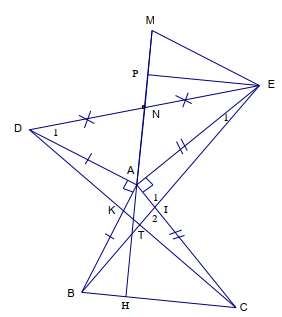
\includegraphics[width=0.4\textwidth]{22-4-lg.png}$$
    Vẽ hình đúng đến câu a
    \begin{enumerate}
        \item Chứng minh được $\Delta \mathrm{DAC}=\Delta \mathrm{BAE}$ (c.g.c )\\[5px]
        $\Rightarrow \mathrm{DC}=\mathrm{BE}$\\[5px]
        Xét $\triangle$ AIE và $\Delta \mathrm{TIC}$ có :\\[5px]
        $\widehat{\mathrm{I}_1}=\widehat{\mathrm{I}_2}(\text { đđ) } \\[5px]
        \mathrm{E}_1=\widehat{\mathrm{C}_1}(\text { do } \Delta \mathrm{DAC}=\Delta \mathrm{BAE}) \\[5px]
        \Rightarrow \widehat{\mathrm{EAI}}=\widehat{\mathrm{CTI}} \\[5px]$
        $\Rightarrow \widehat{\mathrm{CTI}}=90^{\circ}=>\mathrm{DC} \perp \mathrm{BE}$
        \item $\text { Chứng minh được } \Delta \mathrm{MNE}=\Delta \mathrm{AND} \text { (c.g.c) } \\[5px]
        \Rightarrow \widehat{\mathrm{D}_1}=\widehat{\mathrm{MEN}}, \mathrm{AD}=\mathrm{ME} \\[5px]
        \text { mà } \mathrm{AD}=\mathrm{AB}(\mathrm{gt}) \\[5px]
        \Rightarrow \mathrm{AB}=\mathrm{ME}(\text{đpcm})(1) \\[5px]
        \text {Vì } \left.\widehat{\mathrm{D}_1}=\widehat{\mathrm{MEN}}=>\mathrm{DA} / / \mathrm{ME}=>\widehat{\mathrm{DAE}}+\widehat{\mathrm{AEM}}=180^{\circ} \text { ( trong cùng phía }\right) \\[5px]
        \text {mà } \mathrm{BAC}+\widehat{\mathrm{DAE}}=180^{\circ} \\[5px]
        \Rightarrow>\widehat{\mathrm{BAC}}=\widehat{\mathrm{AEM}}(2)$\\[5px]
        Ta lại có: $\mathrm{AC}=\mathrm{AE}$ (gt) (3). Từ (1),(2) và (3) $\Rightarrow \Delta \mathrm{ABC}=\Delta \mathrm{EMA}(đ \mathrm{pcm})$
        \item Kéo dài $\mathrm{MA}$ cắt $\mathrm{BC}$ tại $\mathrm{H}$. Từ $\mathrm{E}$ hạ $\mathrm{EP} \perp \mathrm{MH}$\\[5px]
        Xét $\triangle \mathrm{AHC}$ và $\triangle \mathrm{EPA}$ có:\\[5px]
        $\widehat{\mathrm{CAH}}=\widehat{\mathrm{AEP}}(\text { do cùng phía với góc PAE }) \\[5px]
        \widehat{\mathrm{AE}}=\mathrm{CA}(\mathrm{gt}) \\[5px]
        \Rightarrow \widehat{\mathrm{PAE}}=\widehat{\mathrm{HCA}}(\text { do } \triangle \mathrm{ABC}=\Delta \mathrm{EMA} \text { câu b) } \\[5px]
        \Rightarrow \widehat{\mathrm{EPA}}=\widehat{\mathrm{AHC}} \\[5px]
        \Rightarrow \widehat{\mathrm{AHC}}=90^{\circ} \\[5px]
        \Rightarrow \mathrm{MA} \perp \mathrm{BC}(\text { g.c.g })$
    \end{enumerate}
}
\end{bt}

\begin{bt}
    Một số chính phương có dạng $\overline{a b c d}$. Biết $\overline{a b}-\overline{c d}=1$. Hãy tìm số $\overline{a b c d}$.
\loigiai{
    Ta có $a, b, c$, d là các số nguyên từ 0 đến $9 ; \mathrm{a}, \mathrm{c}$ khác 0\\[5px]
    Là số chính phương nên $\overline{a b c d}=\mathrm{n}^2$ và $\overline{a b}-\overline{c d}=1$\\[5px]
    Hay $\mathrm{n}^2=\overline{a b c d}=100 \overline{a b}+\overline{c d}=100(\overline{c d}+1)+\overline{c d}=101 \overline{c d}+100$\\[5px]
    Suy ra $\mathrm{n}^2-100=(\mathrm{n}-10)(\mathrm{n}+10)=101 \overline{c d}, \mathrm{n}^2$ là số có 4 chữ số vậy $\mathrm{n}<100$ do đó $\mathrm{n}+10=101$\\[5px]
    suy ra $\mathrm{n}=91$ và $\mathrm{n}^2=\overline{a b c d}=91^2=8281$
}
\end{bt}

